\documentclass[12pt, twoside]{article}
\usepackage[letterpaper, margin=1in, headsep=0.5in]{geometry}
\usepackage[english]{babel}
\usepackage[utf8]{inputenc}
\usepackage{amsmath}
\usepackage{amsfonts}
\usepackage{amssymb}
\usepackage{tikz}
\usetikzlibrary{quotes, angles}
\usepackage{graphicx}
\usepackage{enumitem}
\usepackage{multicol}

\newif\ifmeta
\metatrue %print standards and topics tags

\title{Regents Geometry}
\author{Chris Huson}
\date{September 2020}

\usepackage{fancyhdr}
\pagestyle{fancy}
\fancyhf{}
\renewcommand{\headrulewidth}{0pt} % disable the underline of the header
\raggedbottom


\fancyhead[LE]{\thepage}
\fancyhead[RO]{\thepage \\ Name: \hspace{4cm} \,\\}
\fancyhead[LO]{BECA / Dr. Huson / Geometry 09-Congruence-transformations\\* pset ID: 154}

\begin{document}

\subsubsection*{9-3bHW-Transformations}
\begin{enumerate}
\item Apply the translation $(x,y) \rightarrow (x-2,y+4)$ to the point $A(2,-1)$. 
  \begin{center}
    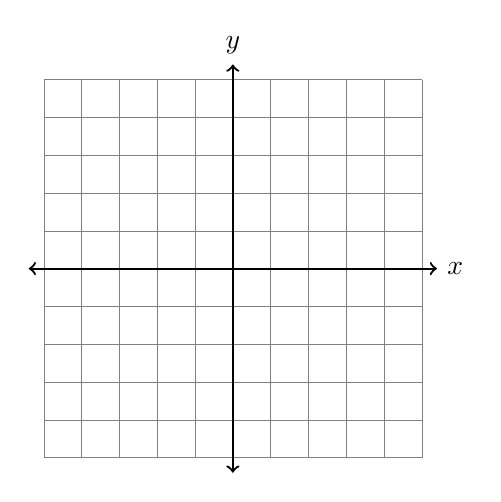
\begin{tikzpicture}[scale=.48]
    \draw [help lines] (-5,-5) grid (5,5);
    \draw [thick, <->] (-5.4,0) -- (5.4,0) node [right] {$x$};
    \draw [thick, <->] (0,-5.4)--(0,5.4) node [above] {$y$};   
  \end{tikzpicture}
\end{center}

\item What is the image of $B(2,4)$ under a reflection across the $x$-axis?
    \begin{center}
      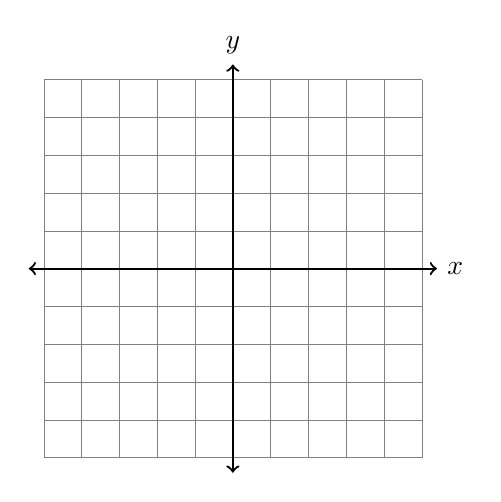
\begin{tikzpicture}[scale=.48]
      \draw [help lines] (-5,-5) grid (5,5);
      \draw [thick, <->] (-5.4,0) -- (5.4,0) node [right] {$x$};
      \draw [thick, <->] (0,-5.4)--(0,5.4) node [above] {$y$};   
    \end{tikzpicture}
  \end{center}

\item State the translation that would map $C(-3,1)$ onto $C'(4,0)$.
    \begin{center}
      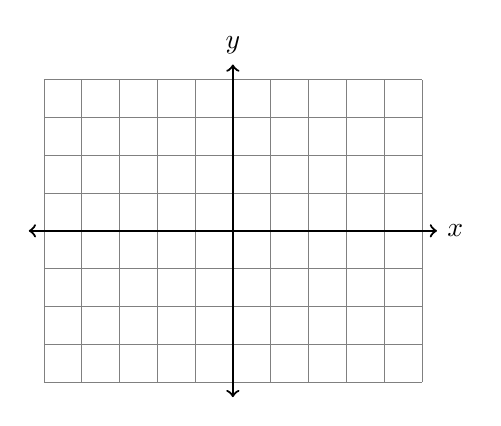
\begin{tikzpicture}[scale=.48]
      \draw [help lines] (-5,-4) grid (5,4);
      \draw [thick, <->] (-5.4,0) -- (5.4,0) node [right] {$x$};
      \draw [thick, <->] (0,-4.4)--(0,4.4) node [above] {$y$};   
    \end{tikzpicture}
  \end{center}

\newpage
\item Given $D(1,9) \rightarrow D'(4,3)$. Find the image of $E(6,-2)$ with the translation.
    \begin{center}
      \begin{tikzpicture}[scale=.48]
      %\draw [help lines] (-5,-5) grid (5,5);
      \draw [thick, <->] (-5.4,0) -- (5.4,0) node [right] {$x$};
      \draw [thick, <->] (0,-5.4)--(0,5.4) node [above] {$y$};   
    \end{tikzpicture}
  \end{center}

\item The image of triangle $ABC$ after a translation is $\triangle A'B'C'$. Is the area of the triangle greater, smaller, or the same after the translation? Justify your answer. \vspace{3cm}

\item On the graph below, draw $\overline{AB}$, with $A(-2,1)$ and $B(6,3)$, labeling the end points. Determine and state the coordinates of the midpoint $M$ of $\overline{AB}$ and mark and label it on the graph.\\
      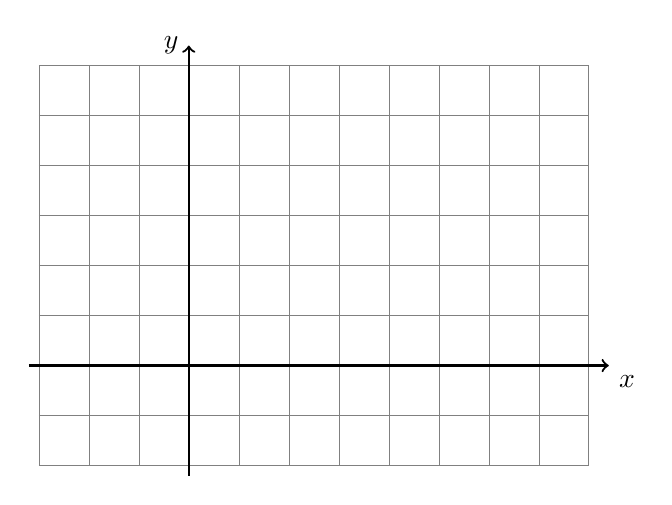
\begin{tikzpicture}[scale=.635]
        \draw [help lines] (-3,-2) grid (8,6);
        \draw [thick, ->] (-3.2,0) -- (8.4,0) node [below right] {$x$};
        \draw [thick, ->] (0,-2.2)--(0,6.4) node [left] {$y$};
      \end{tikzpicture}

\end{enumerate}
\end{document}